\begin{figure*}
    \centering
	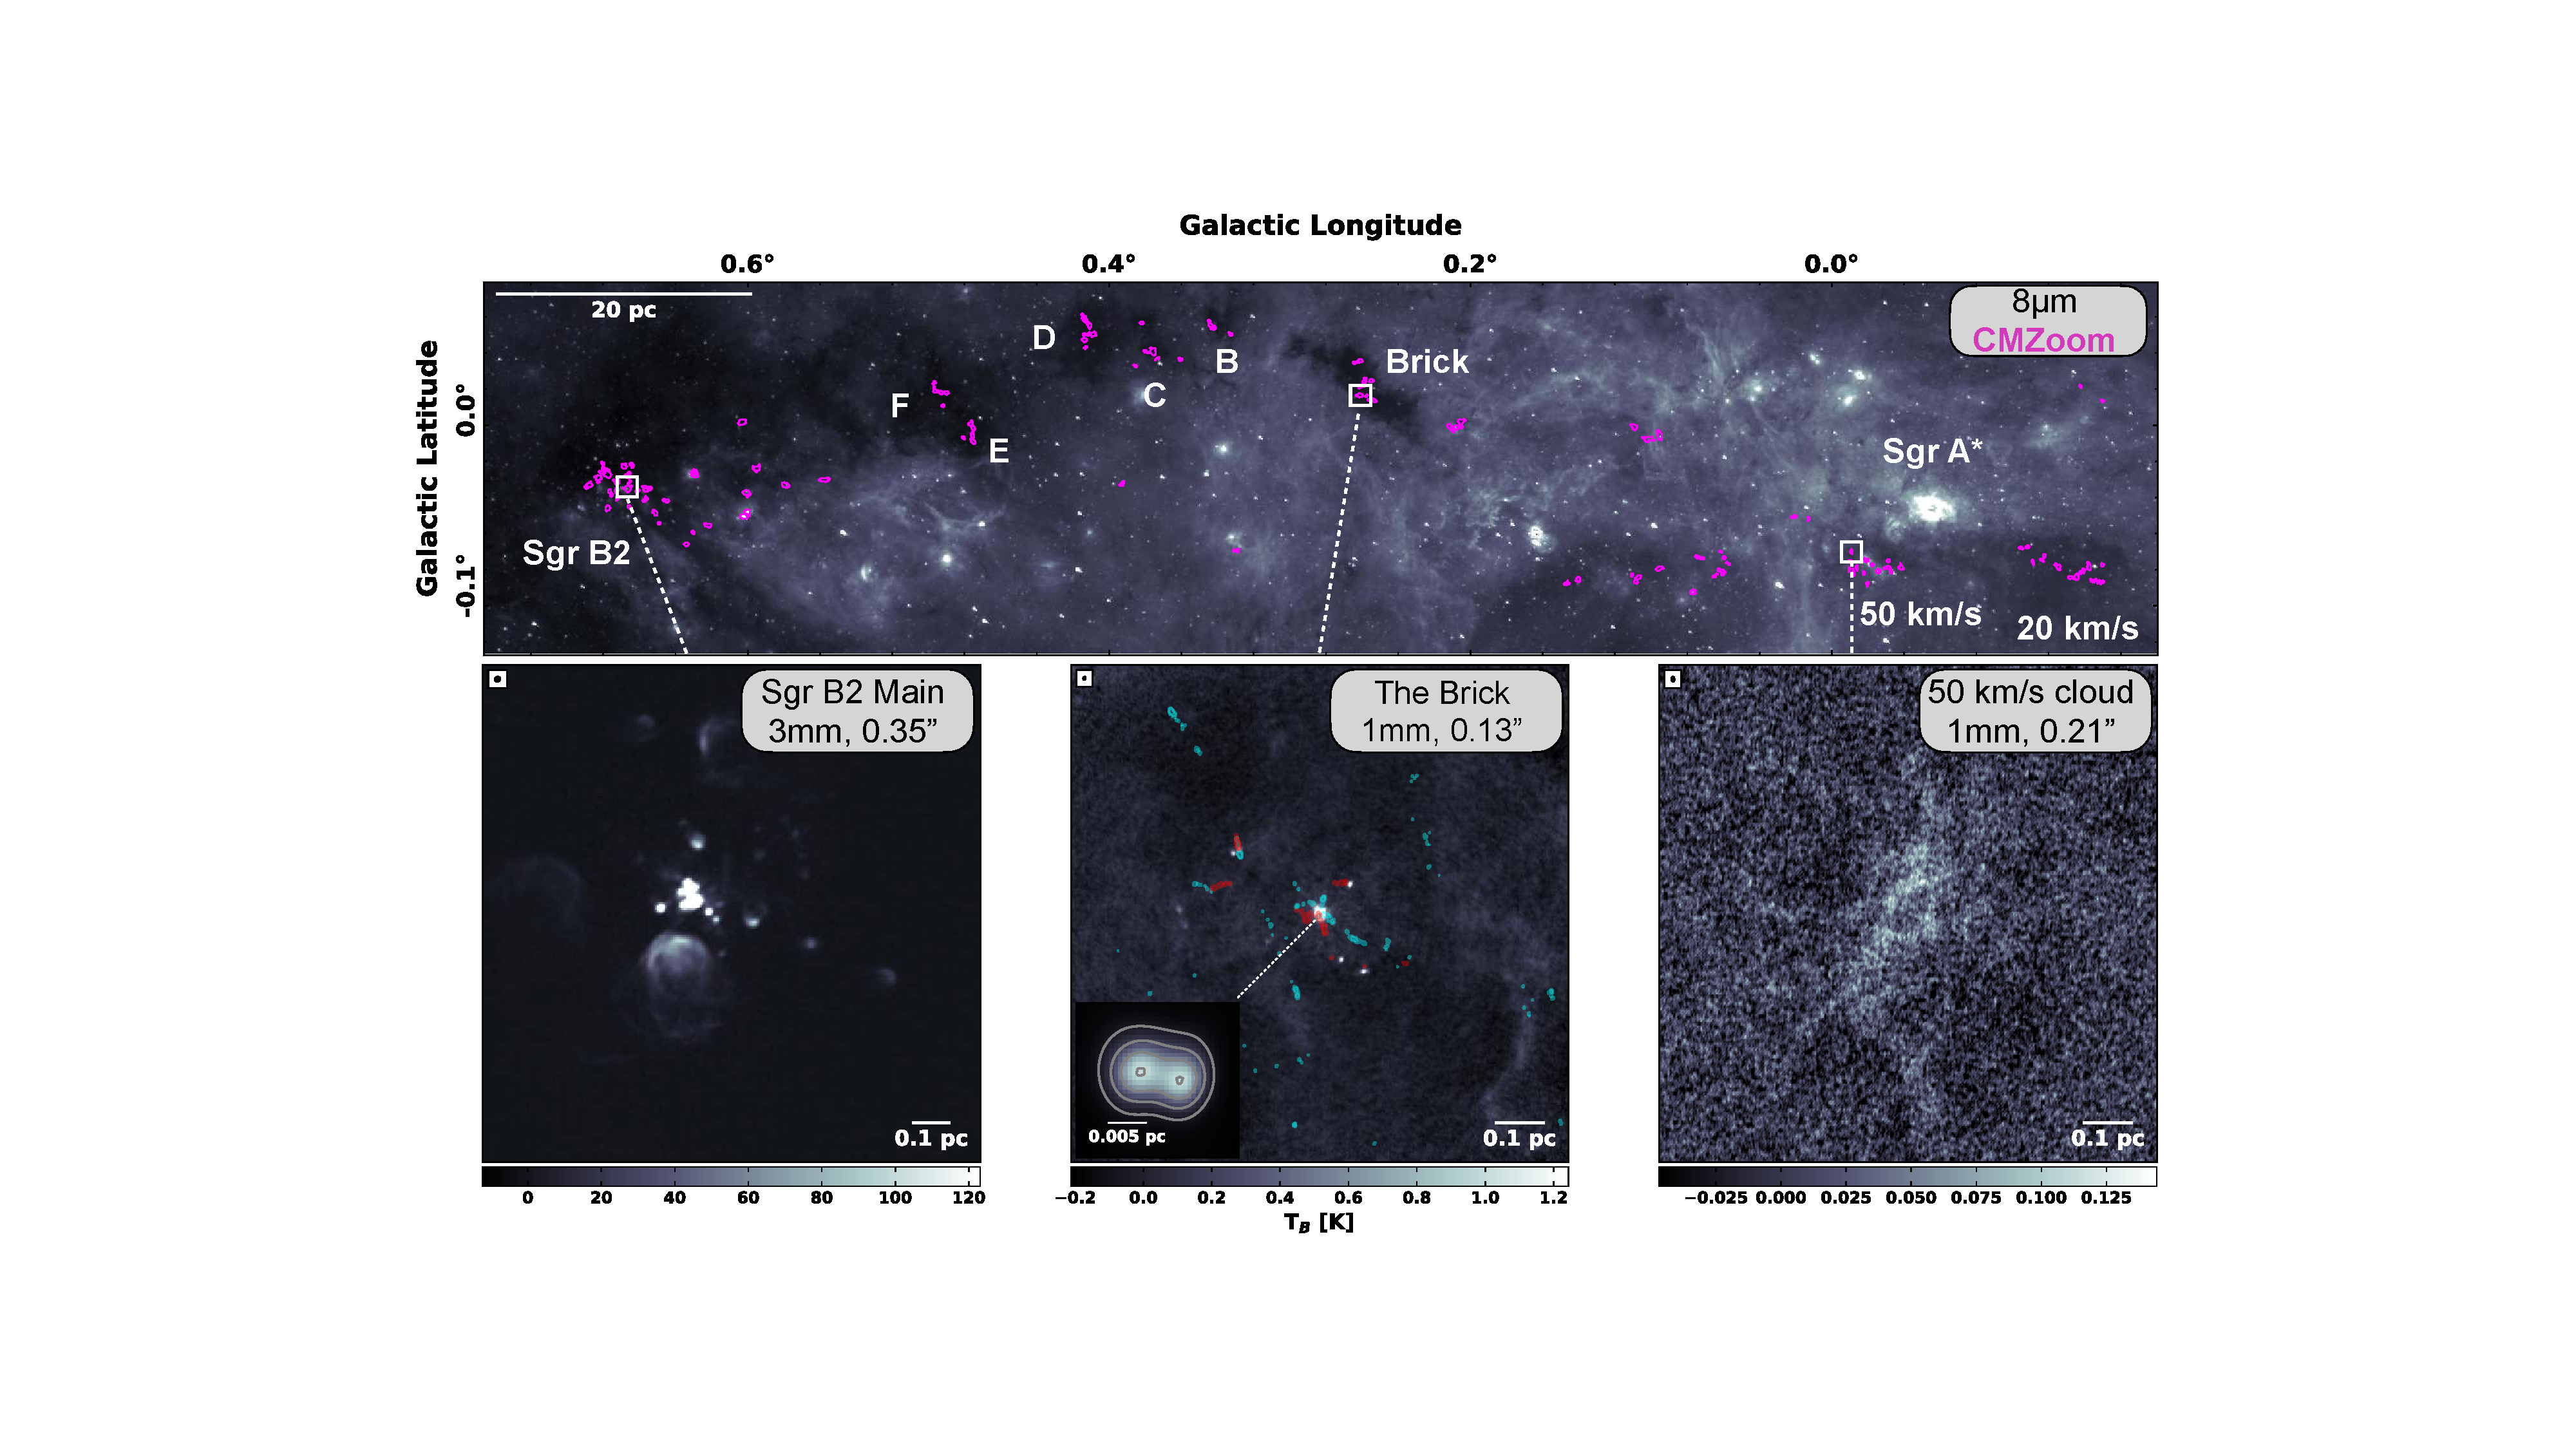
\includegraphics[trim=0 0cm 0 0cm, clip, width=0.95\textwidth]{./figs/high_res_colourbars_compressed.pdf}
    \caption{\textit{Top}: 8~$\mu$m map of a portion of the CMZ \citep{Churchwell2009}. Contours show the 1.3~mm source catalogue from the CMZoom survey \citep{Battersby2020}. \textit{Bottom}: ALMA observations of three regions with differing levels of star-forming activity: from the highly active Sgr B2 Main \citep[\textit{left},][]{Ginsburg2018b}, to the weakly star-forming G0.253+0.016 (the Brick) \citep[\textit{centre},][]{Walker2021}, and the 50~km~s$^{-1}$ cloud, which shows no evidence for embedded protostellar cores \citep[\textit{right},][]{Lu2020}. Blue/red contours in the centre panel show outflows via integrated blue/red-shifted SiO (5-4) emission, and the inset shows the the centre of the field, revealing a protostellar binary with separation $\sim$ 1000~AU.}
    \label{fig:high_res}
\end{figure*}